\documentclass[SSS_Laborbericht.tex]{subfiles}
\usepackage{pdfpages}
\usepackage{listings}

\begin{document}

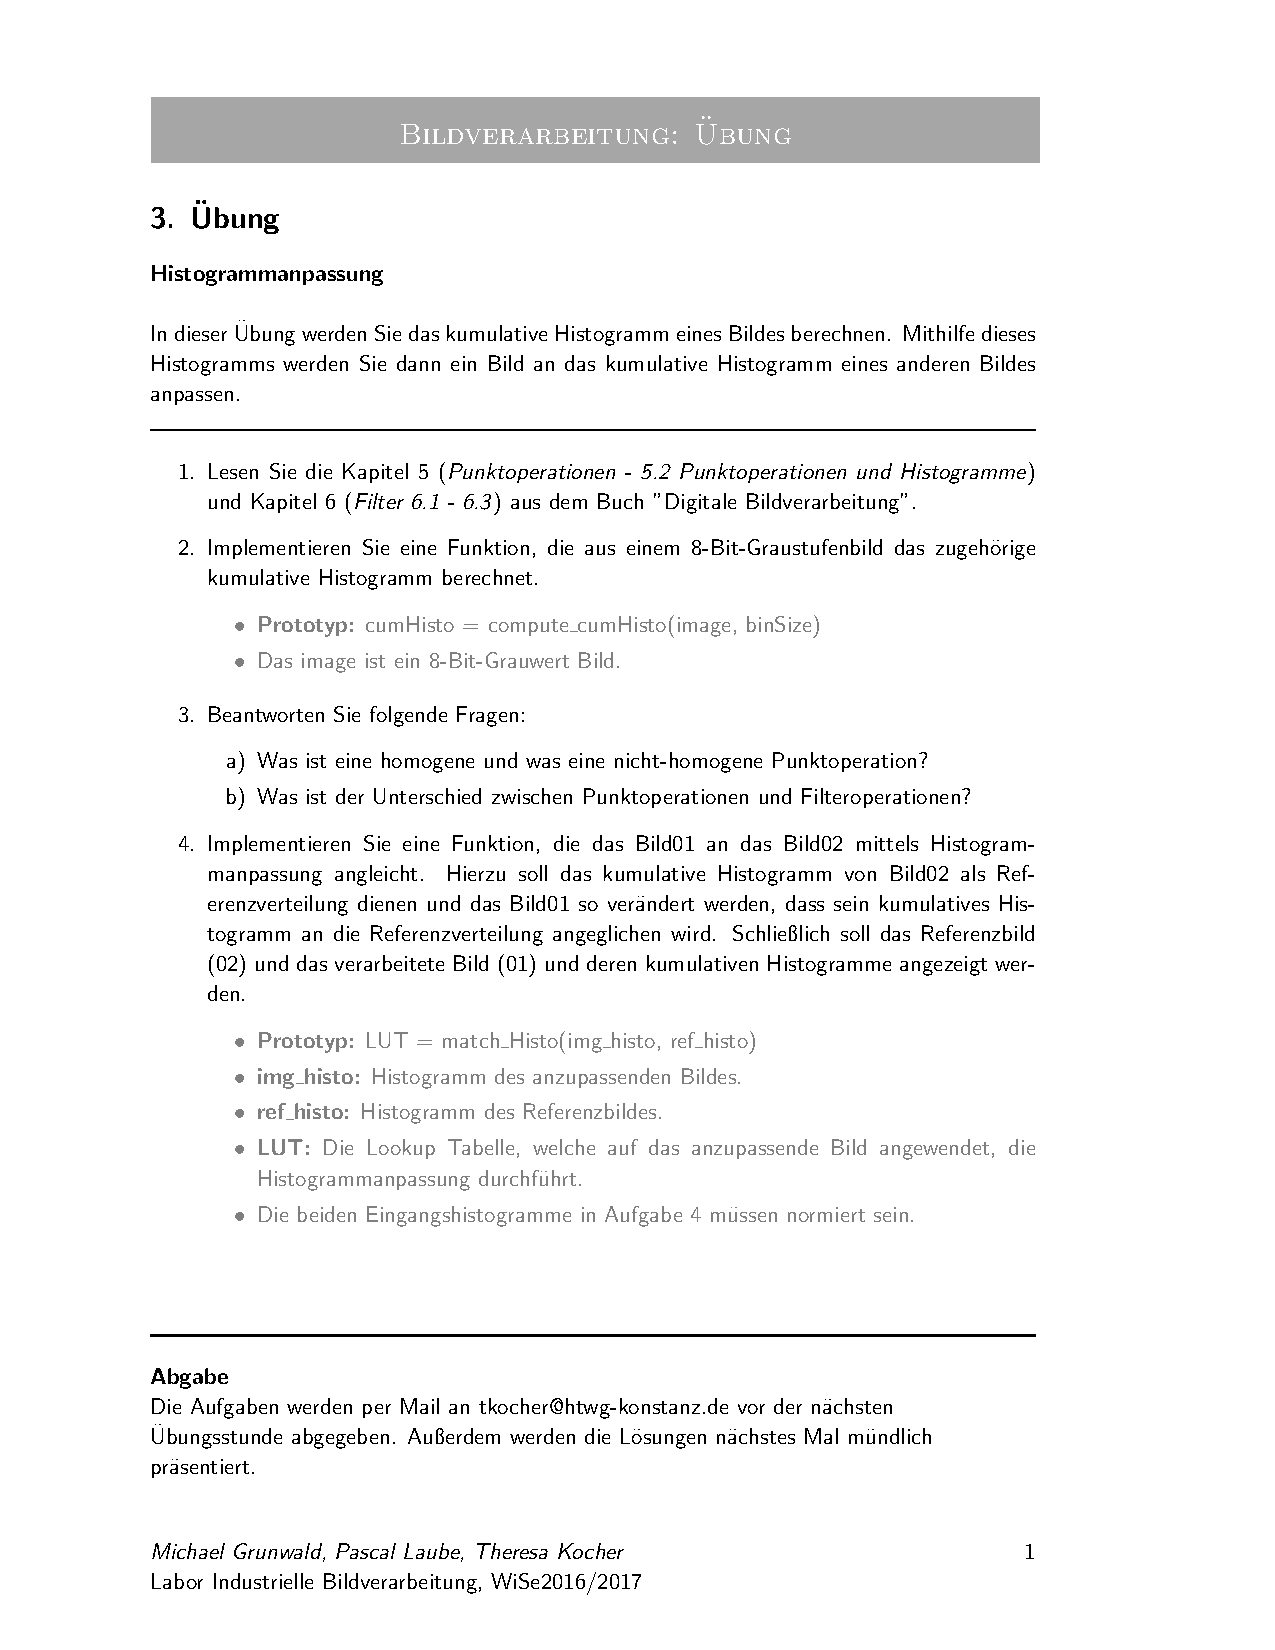
\includepdf[pages={1}]{uebung3.pdf}
\includepdf[pages={2}]{uebung3.pdf}

\noindent\Large{Aufgabe 2}
\lstinputlisting[style=PYTHON, frame=single, caption=rgb2gray, firstline=7, lastline=9, firstnumber=7]{template.py}

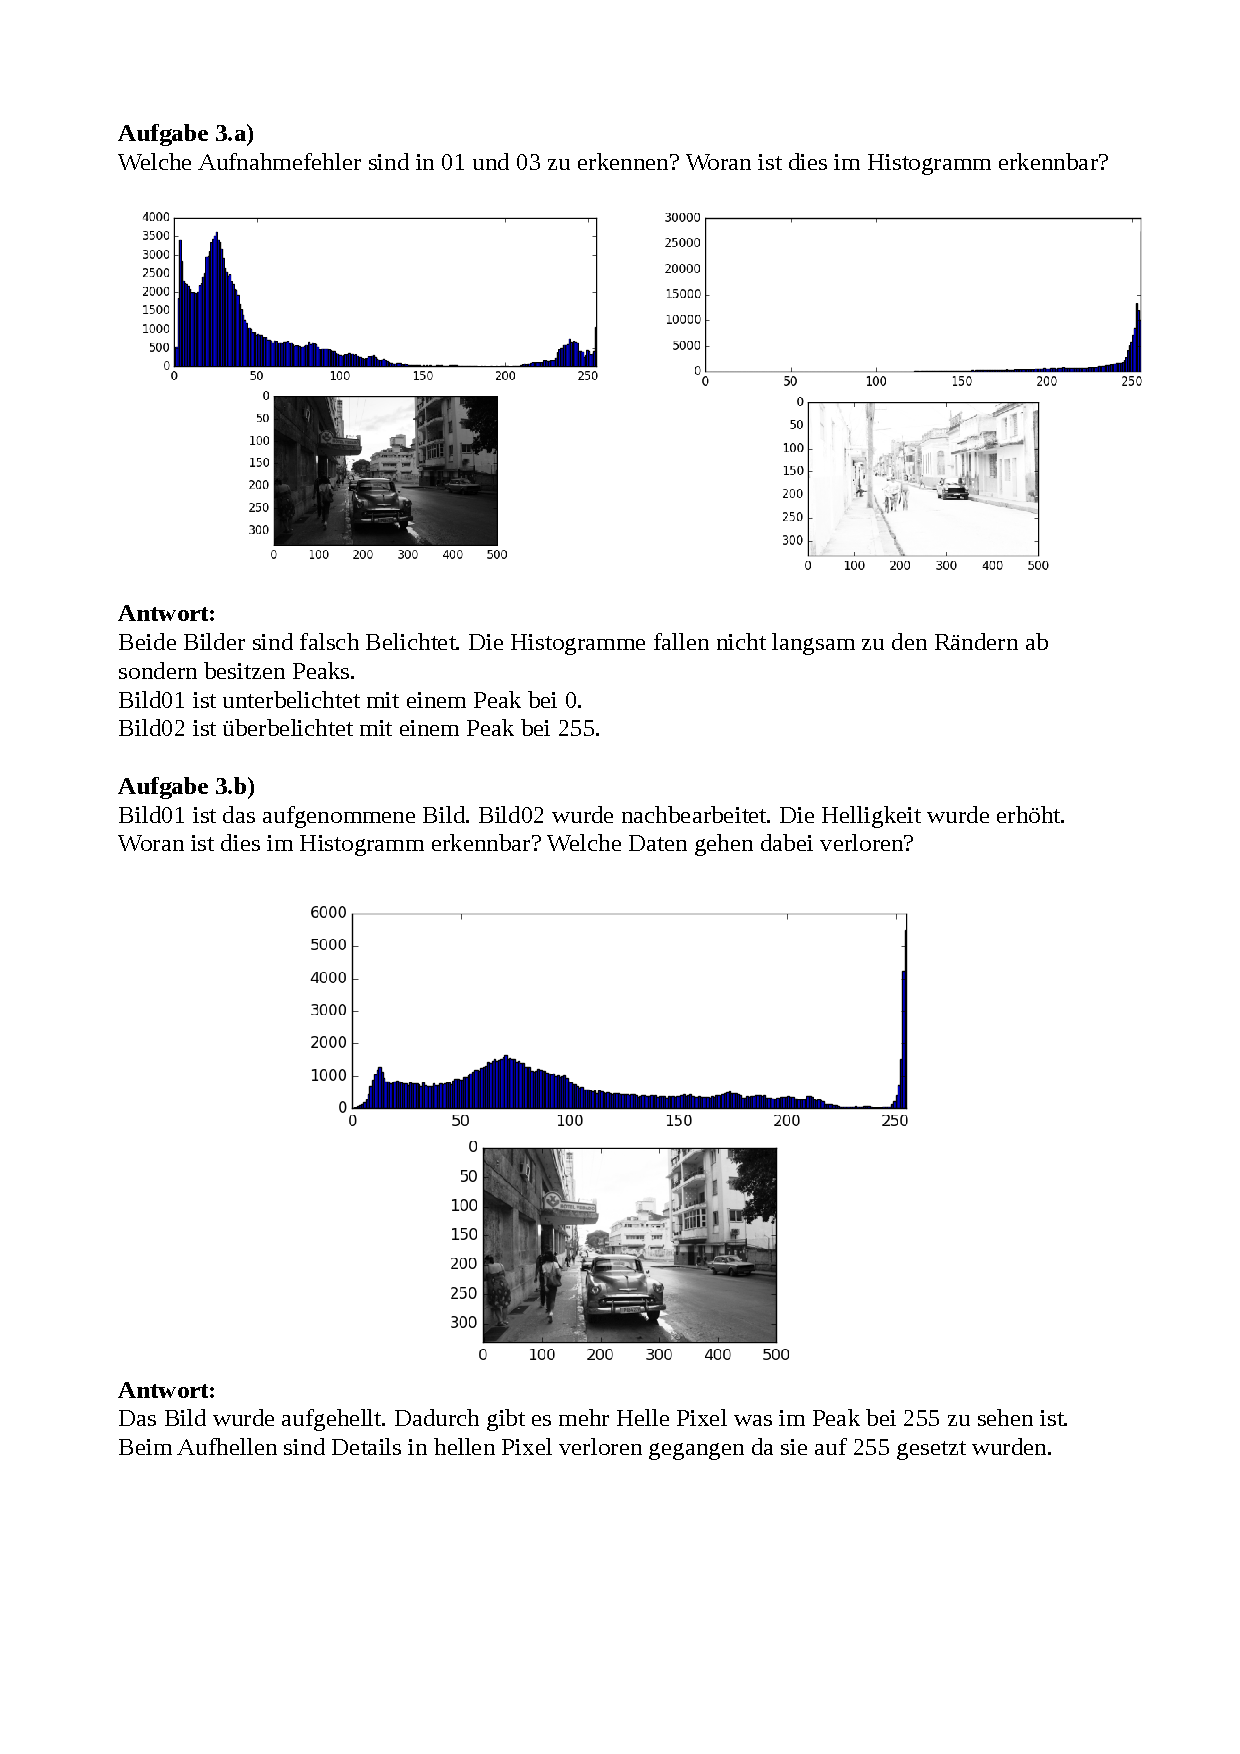
\includepdf[pages={1}]{Aufgabe3.pdf}
\includepdf[pages={2}]{Aufgabe3.pdf}

\newpage
\noindent\Large{Aufgabe 4)}
\noindent\normalsize{Wenn in einem Foto nur dunkle Bereich aufgehellt und helle Bereiche abgedunkelt werden können Details erhalten bleiben.}

\end{document}